\begin{center} \textbf{\huge Methodology} \end{center}
\textbf{\large Batch}\\
The batch or offline model implements a classic Traing-Testing-Phase setup. A subset training points are pre-collected from a stream and used to build a final model on  which three testsets are applied. The batch model functions as a reference model to observe the performance of the initial training over time. \\
For training 600 data points were taken collected in the first three days. The following four days with 1248 data points created the first test set for this model. A second and a third test set where created after the previous testphase and contained 1102 and 1172 data points, respectivly RSS feeds.\\

      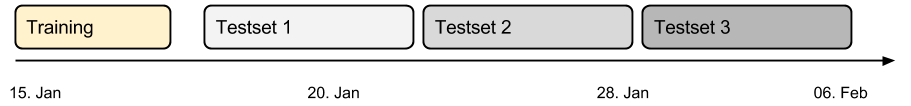
\includegraphics[width=0.24\textwidth]{./time_models/OfflineModel.png}\\
\textbf{\large Bruteforce}\\
On the other hand On-line Learning will change the model with the arriving of new data points.
The bruteforce approach updates the model after a period of time through retraining. Based on a sliding window over the stream with a constant number of data points 
the model is rebuilt. The window size for the bruteforce model contains as well 600 data points. After 1000 test points we retrained it with the last 600 data points arrived. We then waited for 1000 data points and second retrain phase with the same window size followed which was tested also with 1000 new data points.\\

   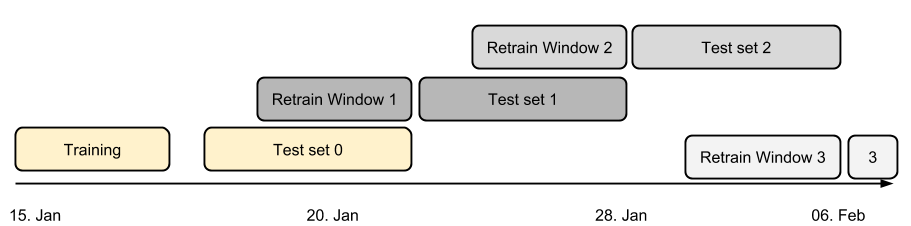
\includegraphics[width=0.2\textwidth]{./time_models/BruteforceModel}\\
\textbf{\large Threshold-triggered}\\
As a variation of the bruteforce model-update the threshold triggered one will rebuild the model on a sliding window as soon as the accuracy of our model is beneth a certain threshold. The window size of the error-triggered model is constructed like the other szenarios out of 600 datapoints. Due to our observations an diserable accurency threshold of 63\% seamed reasonable. A sanity window of testpoints ensures that at least 300 new data points arrive and based on their performance the model is rebuild.\\
\\
\\

   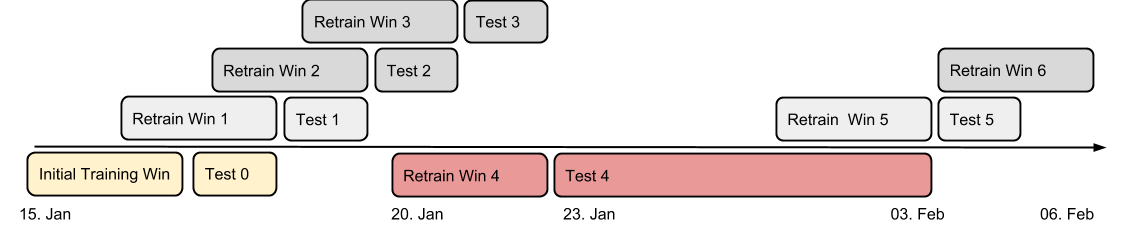
\includegraphics[width=0.2\textwidth]{./time_models/Errortriggered}\\
\textbf{\large Incremental}\\
In the incremental model, unlike the other update models, following an initial training-only phase, all the incoming stream items are always used for training right after the prediction. So, this way the immidiate information whether the prediction was good or bad can be used for improving the model on the fly. In other words, predictive model building and testing phases perfectly overlap in incremental model update method. Updating the model is done by 'dampening' the feature vectors of the past elements. We used incremental model to achieve a real-time response to the changes in the data arguably making the text mining application more resillant to the conceptual drifts.

